\documentclass[graphics]{beamer}

\usepackage{graphicx}
\usepackage{verbatim}
\usepackage{wrapfig}
\useoutertheme{shadow}
%\usecolortheme{orchid}
\usecolortheme{seahorse}


% math commands
\newcommand{\be}{\begin{eqnarray}}
\newcommand{\ee}{\end{eqnarray}}
\newcommand{\beq}{\begin{equation}}
\newcommand{\eeq}{\end{equation}}
\def\simless{\mathbin{\lower 3pt\hbox
      {$\rlap{\raise 5pt\hbox{$\char'074$}}\mathchar"7218$}}}
\def\simgreat{\mathbin{\lower 3pt\hbox
      {$\rlap{\raise 5pt\hbox{$\char'076$}}\mathchar"7218$}}} %> or of order

% variables

\def\toonscale{0.45}
\def\mboxy#1{\mbox{\small #1}}


\begin{comment}
\AtBeginSection[]{
  \frame{
    \frametitle{Outline}
    \tableofcontents[currentsection]
  }
}
\end{comment}

\title{Agile Real Time International Radio Signal Processing
}
\subtitle{interim update}
\author[U. Pen]{Ue-Li Pen
\\[8mm] 
}
\date{May 18, 2016}


\begin{document}

\frame{
%\vspace{-2.3in}
%\begin{center}\hspace{-0.75in} 
%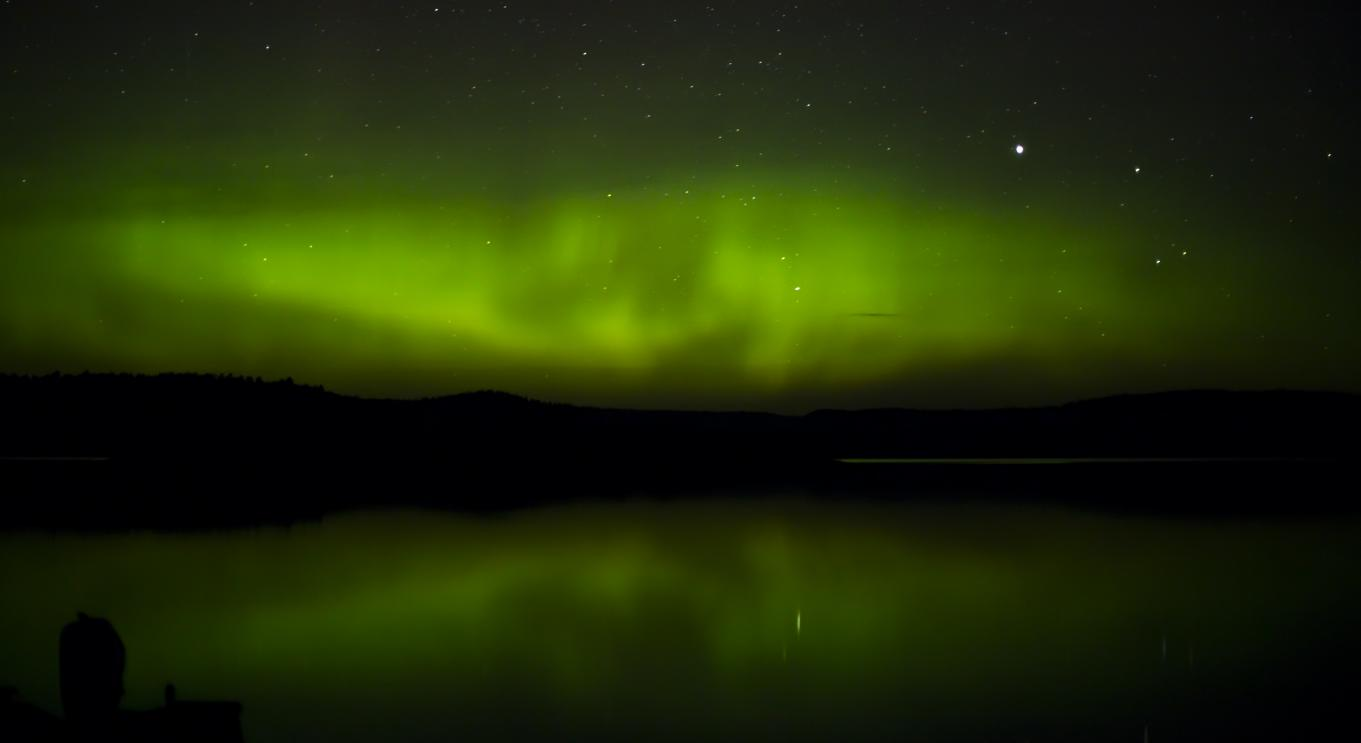
\includegraphics[width=5.4in]{Figures/traverse-aurora.jpg}
%\end{center}
%\vspace{-0.2in}image credit: Andre Recnik
%\vspace{-3in}
\begin{picture}(320,250)
\put(-50,20){
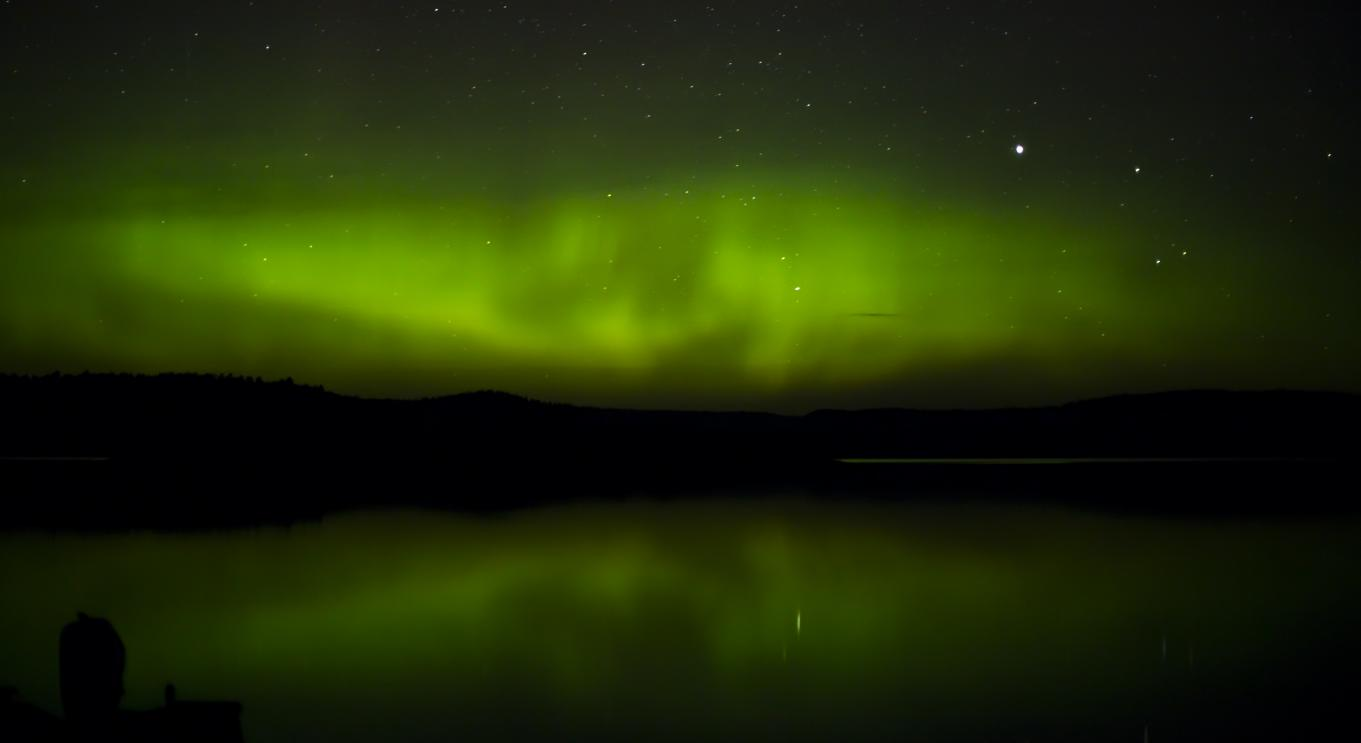
\includegraphics[width=5.5in]{Figures/traverse-aurora.jpg}}
%\textcolor{red}{
image credit: Andre Recnik
\end{picture}
}

%\section*{Introduction}
\section{Project status}

\begin{comment}
  \subsection{Outline}

  \frame{
    \frametitle{Outline}
    \tableofcontents
  }
\end{comment}

  \frame{
\vspace{-0.5in}
    \frametitle{Pulsar VLBI}
    \begin{itemize}
        \item SOSCIP postdoc: Dr I-Sheng Yang, implemented milestone 1
        \item OCE-VIA approved: 
        \item 
%          \vspace{-0.15in}
    \end{itemize}
\vspace{-0.1in}\hspace{.3in}
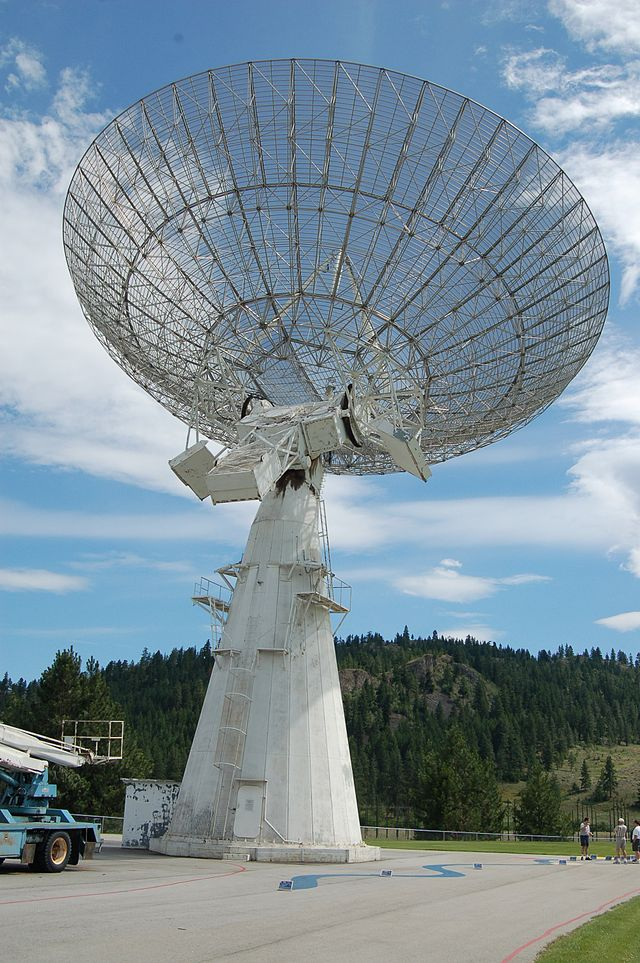
\includegraphics[width=1.2in]{Figures/DRAO_26m_dish.jpg}
\vspace{-0.5in}
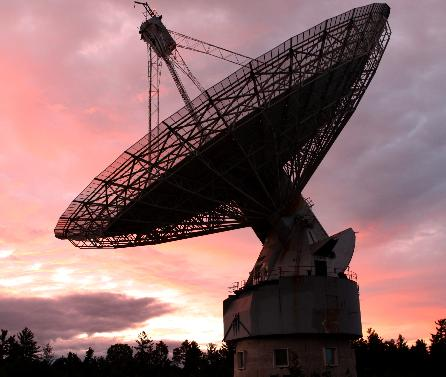
\includegraphics[width=1.9in]{Figures/IMG-7749-ARO-crop.JPG}
  }

  \frame{
\vspace{-0.5in}
    \frametitle{Canadian VLBI fringes!}
    \begin{itemize}
      \item work by Liam Connor, Robert Main
        \item crab giant pulse
        \item April 2016, ARO-DRAO
%          \vspace{-0.15in}
    \end{itemize}
\vspace{-0.1in}\hspace{.3in}
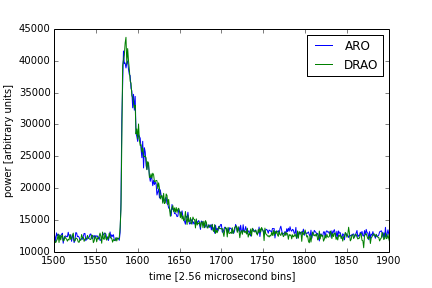
\includegraphics[width=1.9in]{Figures/ARO-DRAO-PulseComp.png}
\vspace{-0.5in}
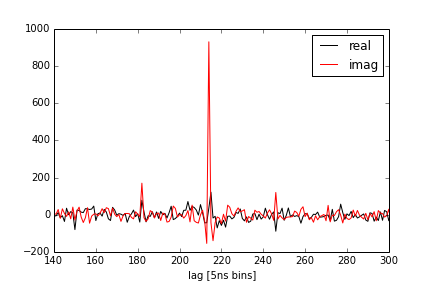
\includegraphics[width=1.9in]{Figures/ARO-DRAO-lf-zoom.png}
  }

  \frame{
    \frametitle{BGQ infrastructure}
    \begin{itemize}
        \item SciNet installed Elemental (parallel linear algebra) for
          data analysis
        \item stuck on numpy/ESSL linkage.
    \end{itemize}
}

\end{document}
